\section{Produktfunktionen}
	% \input{3-Produktfunktionen}

		\subsection{Use Cases}
		% \input{3-1-Use_Cases}

		In dem zu modellierenden System wurden zwei Unterumgebungen (\emph{Server} sowie \emph{RobotUnit}) identifiziert, auf welchen die Aktoren \emph{Taxi-Customer}, \emph{Hospital} und \emph{RobotUnit} verschiedene Anwendungsfälle aufrufen können. Der fiktionale Aktor \emph{User} aggregiert die gemeinsamen Use-Cases von \emph{Taxi-Customer} und \emph{Hospital} \\
		%Die Abbildungen \ref{fig:3-1-server-use-cases} und \ref{fig:3-1-use-cases-robot-unit} stellen die Funktionalitäten dieser Teilsysteme dar.
			\subsubsection{Server}
			Der \emph{Server} stellt das zentrale System dar, über welches die \emph{Orders} der \emph{Taxi-Customer} und des \emph{Hospitals} abgewickelt und an die \emph{Robots} verteilt werden.
				\begin{figure}[H]
					\centering
					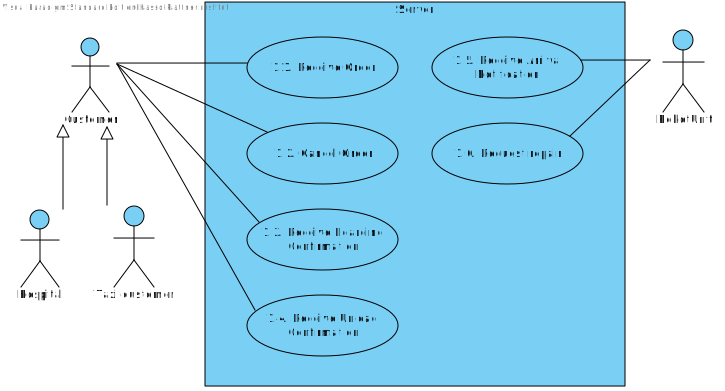
\includegraphics[width=1.0\textwidth]{img/2-Analyse-Server}
					\caption{Use Cases des Teilsystems \emph{Server}}
					\label{fig:3-1-server-use-cases}
				\end{figure}
			\pagebreak
			\subsubsection{RobotUnit}
			Die \emph{RobotUnit} stellt als Kombination des \emph{Robots} sowie der \emph{Robot Software} die ausführende Komponente dar und bietet dem \emph{Server} Möglichkeiten der Steuerung und Informationsabfrage.
				\begin{figure}[H]
					\centering
					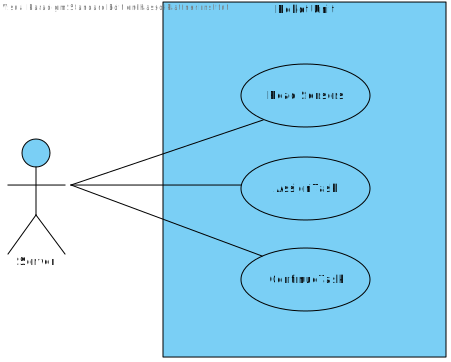
\includegraphics[width=0.8\textwidth]{img/2-Analyse-RobotUnit}
					\caption{Use Cases des Teilsystems \emph{Robot}}
					\label{fig:3-1-use-cases-robot-unit}
				\end{figure}

		\pagebreak

		\subsection{Beschreibungen der Use Cases in der \emph{Server} Umgebung}
			\subsubsection{Beschreibung zu Use Case \emph{1.1}: Receive Order}
			\paragraph*{Charakterisierende Informationen}

			\begin{table}[H]
				\centering
				\begin{tabularx}{\textwidth}{|p{5cm}|X|}
					\hline
					\textbf{Übergeordneter elementarer Geschäftsprozess:} & \emph{Distribute Order}  \\ \hline
					\textbf{Ziel des Use Cases:} & \emph{User} kann eine \emph{Order} (mit unterschiedlicher Dringlichkeit) an den \emph{Server} stellen \\ \hline
					\textbf{Umgebende Systemgrenze:} & \emph{Server} \\ \hline
					\textbf{Vorbedingung:} & \emph{User} verlangt nach einer Transportdienstleistung \\ \hline
					\textbf{Nachbedingung bei erfolgreicher Ausführung:} & \emph{Order} wird ausgeführt, dem anfragenden \emph{User} wird entweder seine Wartelistenposition oder eine Auftragsbestätigung mitgeteilt \\ \hline
					\textbf{Beteiligte Nutzer:} & \emph{User} \\ \hline
					\textbf{Auslösendes Ereignis:} & \emph{User} schickt eine konkrete \emph{Order} an den \emph{Server} \\
					\hline
				\end{tabularx}
			\end{table}

			Über diesen Anwendungsfall können \emph{User} \emph{Orders} über den \emph{Server} an das Personentransportsystem durch stellen.
			Krankenfahrten werden priorisiert. Sollte eine Fahrt auf Anfrage nicht sofort möglich sein, informiert der \emph{Server} den \emph{User} über die Wartelistenposition.

				\paragraph*{Szenario für den Standardablauf (Erfolg)}

				\begin{table}[H]
					\centering
					\begin{tabularx}{\textwidth}{|c|p{2cm}|X|}
					\hline
					Schritt & Nutzer & Beschreibung der Aktivität \\ \hline
					1 & \emph{User} & \emph{User} sendet eine \emph{Order} \\
					2 & \emph{Server} & \emph{Robot} fährt zum \emph{Customer} und führt die \emph{Order} aus  \\
					\hline
					\end{tabularx}
				\end{table}
			\paragraph*{Szenarien für alternative Abläufe\\ (Misserfolg oder Umwege zum Erfolg)}

			\begin{table}[H]
					\centering
					\begin{tabularx}{\textwidth}{|c|p{2cm}|X|}
					\hline
					Schritt & Bedingung für Alternative & Beschreibung der Aktivität \\ \hline
					1 & \mbox{Es ist kein} \emph{Robot} verfügbar & \emph{Server} gibt dem \emph{User} eine Wartelistenposition zurück \\
					\hline
					\end{tabularx}
				\end{table}


			\pagebreak
			%\paragraph*{Beschreibung des allgemeinen Ablaufes}

			\subsubsection{Beschreibung zu Use Case \emph{1.2}: Cancel Order}
			\paragraph*{Charakterisierende Informationen}

			\begin{table}[H]
				\centering
				\begin{tabularx}{\textwidth}{|p{5cm}|X|}
					\hline
					\textbf{Übergeordneter elementarer Geschäftsprozess:} & \emph{Distribute Order} \\ \hline
					\textbf{Ziel des Use Cases:} & \emph{User} kann eine an den \emph{Server} gestellte \emph{Order} zurückziehen \\ \hline
					\textbf{Umgebende Systemgrenze:} & \emph{Server} \\ \hline
					\textbf{Vorbedingung:} & Der \emph{User} überlegt sich, dass er die \emph{Order} stornieren möchte. \\ \hline
					\textbf{Nachbedingung bei erfolgreicher Ausführung:} & Die \emph{Order} wird gelöscht und der \emph{Robot} steht für andere Fahrten wieder zur Verfügung \\ \hline
					\textbf{Beteiligte Nutzer:} & \emph{User} \\ \hline
					\textbf{Auslösendes Ereignis:} & Der \emph{User} storniert seine \emph{Order} \\
					\hline
				\end{tabularx}
			\end{table}

			Der \emph{User} kann seine \emph{Order} stornieren. Ist die zu transportierende Person (\emph{Customer}) zugestiegen, wird die Stornierung ignoriert.

			\paragraph*{Szenario für den Standardablauf (Erfolg)}

			\begin{table}[H]
				\centering
				\begin{tabularx}{\textwidth}{|c|p{2cm}|X|}
					\hline
					Schritt & Nutzer & Beschreibung der Aktivität \\ \hline
					1 & \emph{User} & \emph{User} zieht seine \emph{Order} zurück \\
					2 & \emph{Server} & Der \emph{Server} löscht die \emph{Order} aus der Warteschlange. Ein mit dieser \emph{Order} beschäftigter \emph{Robot} steht daraufhin wieder zur Verfügung \\
					\hline
				\end{tabularx}
			\end{table}


			\pagebreak

			\subsubsection{Beschreibung zu Use Case \emph{1.3.}: Receive Boarding Confirmation}
				\paragraph*{Charakterisierende Informationen}

				\begin{table}[H]
					\centering
					\begin{tabularx}{\textwidth}{|p{5cm}|X|}
						\hline
						\textbf{Übergeordneter elementarer Geschäftsprozess:} & \emph{Take Customer to Destination} \\ \hline
						\textbf{Ziel des Use Cases:} & Dem \emph{Server} signalisieren, dass ein \emph{Customer} zugestiegen ist \\ \hline
						\textbf{Umgebende Systemgrenze:} & \emph{Server} \\ \hline
						\textbf{Vorbedingung:} & Der \emph{Robot} erreicht den \emph {Customer} \\ \hline
						\textbf{Nachbedingung bei erfolgreicher Ausführung:} & Der \emph{Robot} setzt seine Fahrt mit zugestiegenem \emph{Customer} in Richtung der nächsten \emph{Destination} fort \\ \hline
						\textbf{Beteiligte Nutzer:} & \emph{User} \\ \hline
						\textbf{Auslösendes Ereignis:} & Der \emph{User} bestätigt dem \emph{Server}, dass der \emph{Customer} (zu transportierende Person) sich auf dem \emph{Robot} befindet \\
						\hline
					\end{tabularx}
				\end{table}

				Der \emph{Customer} befindet sich auf dem \emph{Robot}. Um die Fahrt fortzusetzen, wird dies dem \emph{Server} mitgeteilt.
					\paragraph*{Szenario für den Standardablauf (Erfolg)}

				\begin{table}[H]
					\centering
					\begin{tabularx}{\textwidth}{|c|p{2cm}|X|}
					\hline
					Schritt & Nutzer & Beschreibung der Aktivität \\ \hline
					1 & \emph{Customer} & \emph{Customer} befindet sich auf dem \emph{Robot}. (\emph{Taxi-Customer} steigt selber zu, ein \emph{Patient} wird von Helfern verladen) \\
					2 & \emph{User} & \emph{User} teilt dem \emph{Server} mit, dass der \emph{Customer} sich auf dem \emph{Robot} befindet \\
					3 & \emph{Server} & \emph{Server} gibt \emph{Robot} den Befehl seine Fahrt in Richtung der nächsten \emph{Destination} fortzusetzen \\
					\hline
					\end{tabularx}
				\end{table}

				%\paragraph*{Beschreibung des allgemeinen Ablaufes}



			\subsubsection{Beschreibung zu Use Case \emph{1.4.}: Receive Unload Confirmation}
				\paragraph*{Charakterisierende Informationen}

				\begin{table}[H]
					\centering
					\begin{tabularx}{\textwidth}{|p{5cm}|X|}
						\hline
						\textbf{Übergeordneter elementarer Geschäftsprozess:} & \emph{Take Customer to Destination} \\ \hline
						\textbf{Ziel des Use Cases:} & Den \emph{Server} informieren, dass \emph{Customer} vom \emph{Robot} abgeladen wurde (im Falle eines \emph{Patients}) , bzw. ausgestiegen ist (im Falle eines \emph{Taxi-Customers}) \\ \hline
						\textbf{Umgebende Systemgrenze:} & \emph{Server} \\ \hline
						\textbf{Vorbedingung:} & \emph{Robot} ist am Ziel angekommen \\ \hline
						\textbf{Nachbedingung bei erfolgreicher Ausführung:} & \emph{Robot} steht für neue \emph{Tasks} zur Verfügung \\ \hline
						\textbf{Beteiligte Nutzer:} & \emph{User} \\ \hline
						\textbf{Auslösendes Ereignis:} & \emph{User} informiert den \emph{Server} darüber, dass sich der \emph{Customer} nicht länger auf dem \emph{Robot} befindet. \\
						\hline
					\end{tabularx}
				\end{table}

				Dieser Use Case dient dazu, den \emph{Server} zu informieren, dass der \emph{Patient} sicher vom \emph{Robot} entfernt wurde, bzw. \emph{Taxi-Customer} ausgestiegen ist. Der \emph{Robot} steht für neue \emph{Tasks} wieder zur Verfügung.

				\paragraph*{Beschreibung des allgemeinen Ablaufes}
					\begin{table}[H]
					\centering
					\begin{tabularx}{\textwidth}{|c|p{2cm}|X|}
					\hline
					Schritt & Nutzer & Beschreibung der Aktivität \\ \hline
					1 & \emph{User} & \emph{Patient} wird vom Roboter entfernt, bzw. \emph{Taxi-Customer} steigt aus \\
					2 & \emph{User} & \emph{User} sendet Nachricht an {Server}, dass sich der \emph{Customer} nicht länger auf dem \emph{Robot} befindet \\
					\hline
					\end{tabularx}
				\end{table}

		\subsubsection{Beschreibung zu Use Case \emph{1.5.}: Receive Arrival Notification}

			\paragraph*{Charakterisierende Informationen}

			\begin{table}[H]
				\centering
				\begin{tabularx}{\textwidth}{|p{5cm}|X|}
				\hline
				\textbf{Übergeordneter elementarer Geschäftsprozess:} & \emph{Take Customer to Destination} \\ \hline
				\textbf{Ziel des Use Cases:} & Ziel ist es, dem \emph{Robot} zu ermöglichen seine Ankunft bei der aktuellen \emph{Destination} dem \emph{Server} mitzuteilen \\ \hline
				\textbf{Umgebende Systemgrenze:} & \emph{Server}\\ \hline
				\textbf{Vorbedingung:} & Der \emph{Robot} erreicht die aktuelle \emph{Destination} \\ \hline
				\textbf{Nachbedingung bei erfolgreicher Ausführung:} & Der \emph{Robot} wartet, bis der \emph{Server} den Befehl zur Weiterfahrt erteilt \\ \hline
				\textbf{Beteiligte Nutzer:} & \emph{Robot}\\ \hline
				\textbf{Auslösendes Ereignis:} & \emph{Robot} teilt dem \emph{Server} mit, dass er die aktuelle \emph{Destination} erreichte \\
				\hline
				\end{tabularx}
			\end{table}

			Der \emph{Robot} erreicht die \emph{Destination} und muss dem \emph{Server} mitteilen, dass er angekommen ist.

			\paragraph*{Szenario für den Standardablauf (Erfolg)}

			\begin{table}[H]
				\centering
				\begin{tabularx}{\textwidth}{|c|p{2cm}|X|}
				\hline
				Schritt & Nutzer & Beschreibung der Aktivität \\ \hline
				1 & Robot & \emph{Robot} informiert \emph{Server}, dass er angekommen ist. \\
				\hline
				\end{tabularx}
			\end{table}

		\subsubsection{Beschreibung zu Use Case \emph{1.6.}: Request Repair}

		\paragraph*{Charakterisierende Informationen}

		\begin{table}[H]
			\centering
			\begin{tabularx}{\textwidth}{|p{5cm}|X|}
				\hline
				\textbf{Übergeordneter elementarer Geschäftsprozess:} & \emph{Take Customer to Destination} \\ \hline
				\textbf{Ziel des Use Cases:} & Ziel ist es, dem \emph{Robot} im Falle einer Kollision Hilfe zu beschaffen \\ \hline
				\textbf{Umgebende Systemgrenze:} & \emph{Server}\\ \hline
				\textbf{Vorbedingung:} & Ein \emph{Robot} kollidiert mit einem \emph{Obstacle} oder einem anderen \emph{Robot} \\ \hline
				\textbf{Nachbedingung bei erfolgreicher Ausführung:} & Der \emph{Robot} wird von einem externen Dienstleiste repariert und steht nach unbestimmter Zeit wieder zur Verfügung \\ \hline
				\textbf{Beteiligte Nutzer:} & \emph{RobotUnit}\\ \hline
				\textbf{Auslösendes Ereignis:} & \emph{Robot} fordert beim \emph{Server} Hilfe nach einer Kollision an \\
				\hline
			\end{tabularx}
		\end{table}

		Trotz vorsichtigen Fahrens kann es zu Kollisionen kommen, in diesem Falle kann der \emph{Robot} Hilfe beim \emph{Server} beantragen.

		\paragraph*{Szenario für den Standardablauf (Erfolg)}

		\begin{table}[H]
			\centering
			\begin{tabularx}{\textwidth}{|c|p{2cm}|X|}
				\hline
				Schritt & Nutzer & Beschreibung der Aktivität \\ \hline
				1 & Robot & \emph{Robot} informiert \emph{Server} über eine Kollision \\
				1 & Server & \emph{Server} beschafft dem \emph{Robot} Hilfe mittels eines externen Dienstleisters, welcher den \emph{Robot} repariert \\
				\hline
			\end{tabularx}
		\end{table}

				\pagebreak
		\subsection{Beschreibungen der Use Cases in der \emph{RobotUnit} Umgebung}
			\subsubsection{Beschreibung zu Use Case \emph{2.1.}: Read Sensors}

				\paragraph*{Charakterisierende Informationen}

				\begin{table}[H]
					\centering
					\begin{tabularx}{\textwidth}{|p{5cm}|X|}
						\hline
						\textbf{Übergeordneter elementarer Geschäftsprozess:} & \emph{Choose Robot} \\ \hline
						\textbf{Ziel des Use Cases:} & \emph{Robot} kann über seinen Akkustand, seine Position und seine derzeitige \emph{Destination} Auskunft geben\\ \hline
						\textbf{Umgebende Systemgrenze:} & \emph{RobotUnit} \\ \hline
						\textbf{Vorbedingung:} & \emph{Robot} hat eine Anfrage vom \emph{Server} erhalten \\ \hline
						\textbf{Nachbedingung bei erfolgreicher Ausführung:} & \emph{Robot} schickt die ermittelten Informationen an den \emph{Server} \\ \hline
						\textbf{Beteiligte Nutzer:} & \emph{Robot} \\ \hline
						\textbf{Auslösendes Ereignis:} & \emph{Robot} hat eine Anfrage vom \emph{Server} erhalten, seine Sensoren zu lesen und sie dem \emph{Server} zu schicken \\
						\hline
					\end{tabularx}
				\end{table}

				Im Rahmen vom Geschäftsprozess \emph{Choose Robot} sammelt der \emph{Server}
				Informationen über jeden \emph{Robot}. Diese Informationen (z.B
				Akkustand, aktuelle Position, ob der \emph{Robot} gerade ein Ziel verfolgt)
				kann der \emph{Robot} von seinen Hardware-Schnittstellen anfordern. Dieser
				Use Case wird dann ausgefüht, wenn der \emph{Robot} eine Anfrage vom
				Server erhält, seine Sensoren zu lesen, und endet damit, dass der \emph{Robot}
				die zusammengefassten Informationen an den \emph{Server} schickt.

				\paragraph*{Szenario für den Standardablauf (Erfolg)}

				\begin{table}[H]
					\centering
					\begin{tabularx}{\textwidth}{|c|p{2cm}|X|}
						\hline
						Schritt & Nutzer & Beschreibung der Aktivität \\ \hline
						1 & Robot & \emph{Robot} erhält Anfrage vom \emph{Server} \\
						2 & Robot & \emph{Robot} sammelt Informationen von seiner Hardwareschnittstelle und fasst sie zusammen \\
						3 & Robot & \emph{Robot} schickt zusammengefasste Informationen an den Server \\
						\hline
					\end{tabularx}
				\end{table}

				%\paragraph*{Beschreibung des allgemeinen Ablaufes}

				\pagebreak

			\subsubsection{Beschreibung zu Use Case \emph{2.2.}: Perform Task}

				\paragraph*{Charakterisierende Informationen}

				\begin{table}[H]
					\centering
					\begin{tabularx}{\textwidth}{|p{5cm}|X|}
						\hline
						\textbf{Übergeordneter elementarer Geschäftsprozess:} & \emph{Take Customer to Destination} \\ \hline
						\textbf{Ziel des Use Cases:} & \emph{Robot} den \emph{Task} (die \emph{Destinations}) zuweisen\\ \hline
						\textbf{Umgebende Systemgrenze:} & \emph{RobotUnit} \\ \hline
						\textbf{Vorbedingung:} & \textit{ \glqq Choose Robot \grqq } hat den am besten geeigneten \emph{Robot} gefunden und ausgewählt\\ \hline
						\textbf{Nachbedingung bei erfolgreicher Ausführung:} & Ausgewählter \emph{Robot} steuert die erste \emph{Destination} an\\ \hline
						\textbf{Beteiligte Nutzer:} & \emph{Server} \\ \hline
						\textbf{Auslösendes Ereignis:} & Im Use-Case \textit{ \glqq choose Robot \grqq } wurde ein passender \emph{Robot} ausgewählt. Diesem soll nun die \emph{Task} übermittelt werden. \\
						\hline
					\end{tabularx}
				\end{table}

				Dem \emph{Server} wird hiermit die Möglichkeit gegeben, dem \emph{Robot} eine beliebige \emph{Task} zuzuweisen. Es ist möglich den Robot hierrüber zum Abbruch der aktuellen \emph{Task} aufzufordern.

				\paragraph*{Szenario für den Standardablauf (Erfolg)}

				\begin{table}[H]
					\centering
					\begin{tabularx}{\textwidth}{|c|p{2cm}|X|}
						\hline
						Schritt & Nutzer & Beschreibung der Aktivität \\ \hline
						1 & Server & \emph{Server} überträgt ausgewähltem \emph{Robot} den \emph{Task} \\
						2 & Robot & \emph{Robot} führt den \emph{Task} aus \\
						3 & Robot & \emph{Robot} fährt zur \emph{Charging Station}, falls der Akkustand unter einem spezifischem Schwellwert liegt\\
						\hline
					\end{tabularx}
				\end{table}

				%\paragraph*{Beschreibung des allgemeinen Ablaufes}

				\pagebreak


			\subsubsection{Beschreibung zu Use Case \emph{2.3.}: Continue Task}

			\paragraph*{Charakterisierende Informationen}

			\begin{table}[H]
				\centering
				\begin{tabularx}{\textwidth}{|p{5cm}|X|}
					\hline
					\textbf{Übergeordneter elementarer Geschäftsprozess:} & \emph{Take Customer to Destination}  \\ \hline
					\textbf{Ziel des Use Cases:} & \emph{Robot} soll seinen Weg zur nächsten \emph{Destination} seiner aktuellen \emph{Task} fortsetzen \\ \hline
					\textbf{Umgebende Systemgrenze:} & \emph{RobotUnit} \\ \hline
					\textbf{Vorbedingung:} & \emph{Robot} hat seine aktuelle \emph{Destination} erreicht \\ \hline
					\textbf{Nachbedingung bei erfolgreicher Ausführung:} & \emph{Robot} fährt seine nächste \emph{Destination} seiner aktuellen \emph{Task} an \\ \hline
					\textbf{Beteiligte Nutzer:} & \emph{Server} \\ \hline
					\textbf{Auslösendes Ereignis:} & \emph{Server} schickt konkrete Anweisung weiterzufahren an den \emph{Robot} \\
					\hline
				\end{tabularx}
			\end{table}

			Der \emph{Robot} wartet nach Erreichen der aktuellen \emph{Destination} auf eine Benachrichtigung vom \emph{Server}, die ihn zur Weiterfahrt zur nächsten \emph{Destination} seiner aktuellen \emph{Task} auffordert. In diesem Zeitraum ist bpsw. das Beladen des \emph{Robots} mit einem \emph{Patient} möglich.

			%\paragraph*{Beschreibung des allgemeinen Ablaufes}
